%  LaTeX support: latex@mdpi.com
%  In case you need support, please attach all files that are necessary for compiling as well as the log file, and specify the details of your LaTeX setup (which operating system and LaTeX version / tools you are using).

%=================================================================
% \documentclass[energies,article,submit,moreauthors,pdftex]{Definitions/mdpi}
\documentclass[preprints,article,accept,moreauthors,pdftex]{Definitions/mdpi}

%=================================================================
\firstpage{1}
\makeatletter
\setcounter{page}{\@firstpage}
\makeatother
\pubvolume{xx}
\issuenum{1}
\articlenumber{5}
\pubyear{2020}
\copyrightyear{2020}
%\externaleditor{Academic Editor: name}
\history{Received: date; Accepted: date; Published: date}
%\updates{yes} % If there is an update available, un-comment this line

%% MDPI internal command: uncomment if new journal that already uses continuous page numbers
%\continuouspages{yes}


%=================================================================
% Add packages and commands here. The following packages are loaded in our class file: fontenc, inputenc, calc, indentfirst, fancyhdr, graphicx,epstopdf, lastpage, ifthen, lineno, float, amsmath, setspace, enumitem, mathpazo, booktabs, titlesec, etoolbox, tabto, xcolor, soul, multirow, microtype, tikz, totcount, amsthm, hyphenat, natbib, hyperref, footmisc, url, geometry, newfloat, caption

%=================================================================
%% Please use the following mathematics environments: Theorem, Lemma, Corollary, Proposition, Characterization, Property, Problem, Example, ExamplesandDefinitions, Hypothesis, Remark, Definition, Notation, Assumption
%% For proofs, please use the proof environment (the amsthm package is loaded by the MDPI class).

%=================================================================
% Full title of the paper (Capitalized)
\Title{Design, Implementation, and Evaluation of Open Power Quality}

% Authors, for the paper (add full first names)
\Author{Anthony J. Christe, Sergey Negrashov and Philip M. Johnson}

% Authors, for metadata in PDF
\AuthorNames{Anthony J. Christe, Sergey Negrashov and Philip M. Johnson}

% Affiliations / Addresses (Add [1] after \address if there is only one affiliation.)
\address{%
Department of Information and Computer Sciences\\
University of Hawaii at Manoa\\
Honolulu, HI 96822\\
johnson@hawaii.edu}

% Abstract (single paragraph, 200 words max, background, methods, results, conclusions. Currently 193 words.)

\abstract{Modern electrical grids are transitioning from a centralized generation architecture to an architecture which must accomodate distributed, intermittent generation.  This transition also means that the formerly sharp distinction between energy producers (i.e. utility companies) and consumers (residences, businesses, etc) are blurring: residences can now both produce and consume energy, making energy policy more complex. The Open Power Quality (OPQ) project began in 2013 with the goal of designing and implementing a low cost, distributed power quality sensor network in order to provide make useful information about electrical grids available to producers, consumers, and policy makers.  Since then, we have designed low cost hardware devices that monitor power quality  and low-cost cloud-based software services that can economically analyze the data and detect a variety of anomalies. In 2019, we performed a pilot study where 15 OPQ hardware devices were deployed across the University of Hawaii microgrid for three months.  Results of the pilot study provide evidence that OPQ provides a variety of useful monitoring services and that the system could be scaled to service larger geographic regions. We conclude that OPQ provides a new and useful approach to power quality monitoring.}

% Keywords
\keyword{Power Quality, Open Source, Renewable Energy, Grid Stability}


\begin{document}

\section{Introduction}

%{\em The introduction should briefly place the study in a broad context and highlight why it is important. It should define the purpose of the work and its significance. The current state of the research field should be reviewed carefully and key publications cited. Please highlight controversial and diverging hypotheses when necessary. Finally, briefly mention the main aim of the work and highlight the principal conclusions.}

\subsection{Motivation}

Power quality is not currently a concern for most people in developed nations. Just like most people in developed nations assume that their tap water is of adequate quality to drink, most also assume that their electricity is of adequate quality to power their homes and appliances without causing harm. And, in both cases, most people assume that public utilities will appropriately monitor and correct any quality problems if they occur.

Successfully maintaining adequate power quality and providing sufficient amounts of it to meet the rising needs of consumers has been a triumph of electrical utilities for over 100 years. In recent times, however, there have been changes to the nature of electrical generation and consumption that make power quality of increasing concern and interest. First, there is a global need to shift to renewable energy sources. Second, traditional top-down grid power quality monitoring may not be well suited to bottom-up, distributed generation associated with renewable energy sources such as roof-top solar. Third, modern consumer electronics place more stringent demands on power quality.  Finally, effective public policy making in this modern context can be aided by public access to power quality data.  Let's look at each of these in a bit more detail.

{\em 1. We need more renewable energy.} Concerns including pollution, environmental degradation, and climate change have produced a global movement away from centralized, fossil-fuel based forms of electrical energy generation and toward distributed, renewable alternatives such as wind and solar. But the economic, environmental, and political advantages of renewable energy comes with significant new technical challenges. Wind and solar are intermittent (for example, solar energy cannot be harvested at night) and unpredictable (for example, wind and solar energy fluctuate based upon cloud cover and wind speed). In addition, renewable energy generation is often distributed throughout the grid (such as in the case of residential rooftop photovoltaic (PV) systems).

One impact of adding renewable energy generation to an electrical grid is that maintaining adequate power quality is much more challenging. This problem is inversely proportional to the size of the electrical grid. For example, each island in the State of Hawaii maintains its own electrical grid, ranging from a 1.8 GW grid for the island of Oahu to a 6 MW grid for the island of Molokai.  (In contrast, the size of the European electrical grid is approximately 600 GW and the size of the U.S. continental grid is over 1000 GW.) For small grids, the unpredictable nature of power generation by distributed, intermittent renewables can quickly create problems for grid stability. In the case of Hawaii, consumer demand for grid-tied rooftop solar exceeded the ability of Hawaiian Electric to manage, resulting first in complex and expensive "interconnection studies" \cite{trabish_solar_2014,anastasi_energy_2009}, and later in the requirement for new installations to include batteries and grid-disconnected operation.

{\em 2. Traditional top-down monitoring is not well-suited to bottom-up energy generation.} For traditional grid architectures where generation is centralized and under the complete control of the utility, it is common to monitor power quality only to the substation level, because it can be assumed that the power quality experienced at the substation is a reasonably accurate proxy for the power quality experienced by the 1,000 or so end-users serviced by the substation. Furthermore, if an end-user experiences a power quality problem not experienced by the substation, then it is mostly likely due to equipment or electrical issues local to that end-user and not a grid-level problem.

These assumptions might not hold in grids with distributed, intermittent generation by end-users, such as is the case with roof top solar. In these cases, the unpredictable nature of generation can lead to local power quality problems that are not experienced by the substation, and that are not due to any single individual, but rather the bottom-up power generation architecture of the grid. Nakafuji notes that Hawaiian Electric is contending with PV penetrations in excess of 60\% on certain distribution circuits, for which traditional rules of thumb for design of protection and distribution systems might not hold \cite{nakafuji_back--basics_2011}.

{\em 3. Consumer electronics require higher quality power.} The rise of consumer electronics has raised the bar for what constitutes ``adequate" power quality. Only a few decades ago, computers were a rare presence outside of labs and large institutions. Today, computers are everywhere: embedded in phones, washers, refrigerators, thermostats, and so forth. These electronic devices not only have higher power quality requirements, but some of them actually introduce power quality problems in the form of harmonic distortion. Poor power quality can result in electronic devices failing unpredictably, and/or decreasing their lifespan.

{\em 4. Power quality data should be publicly available.} Electrical utilities are not required to be totally transparent about the quality of power they provide to consumers. For example, in Hawaii, utilities are required to make a "best effort" to provide non-harmful voltage and frequency values, but are only required to publicly report on power outages of more than 3 minutes. There is no requirement for utilities to report potentially harmful levels of voltage, frequency, THD, or transients as long as they do not lead to outages. Indeed, in places like Hawaii, there is not yet infrastructure in place to enable utilities to collect that information, even if they were asked to report on it.

Providing power quality data to address the above issues requires solving several difficult technical problems. First, monitoring below the substation level increases the number of required monitoring devices by two to three orders of magnitude. This has significant implications for the cost of monitoring in terms of the devices, and the sheer amount of low-level power quality data that will be produced. Second, this low-level data must be processed in a manner that does not require inordinate amounts of processing, network bandwidth, or storage. Finally, collecting the data is not useful if it cannot be converted into actionable information in a reasonable amount of time.

\subsection{Goals of the Open Power Quality Project}

The goal of the OPQ Project is to provide a scalable source of actionable power quality data about electrical grids, particularly those with high levels of distributed, intermittent power generation. OPQ accomplishes this through the design and implementation of a low-cost sensor network for power quality using custom power quality monitors with real-time, two way communication to a set of cloud-based services. An OPQ sensor network is designed to be useful to consumers who want to better understand the performance of their public utilities, to researchers who wish to design improvements to grid management, and to public policy makers responsible for designing and implementing regulatory frameworks for electrical utilities.  There are several key features of our project emerge from these goals.

{\em OPQ Box.} First, our custom power quality monitoring hardware device, called "OPQ Box" can be produced for approximately US\$75. This is from 10 to 100 times less expensive than commercial power quality monitors. This cost differential means, for example, that instead of monitoring power quality at the level of individual buildings, OPQ makes it economically feasible to monitor power quality on each floor or even in each room of a building. Similarly, instead of monitoring power quality at the substation level of the grid, OPQ Boxes make it feasible to deploy dozens or hundreds into a community to obtain fine-grained data about the impact of solar or other renewables as directly perceived by the customer.

{\em Cloud-native information architecture.} Second, our information architecture is "cloud native", which means that OPQ Boxes are not designed for stand-alone, autonomous use, unlike current commercially available power quality monitors. Instead, our hardware boxes and cloud-based services perform real-time, two-way communication over the Internet to determine what power quality data must be gathered and with what fidelity in order to most efficiently produce actionable information. Two-way communication between the OPQ Boxes and could services creates the ability to control individual OPQ Boxes based upon the global state of all OPQ Boxes in an OPQ sensor network. As a result, OPQ cloud services can obtain and analyze high fidelity wave form data only when desired, without the prohibitive network overhead of constantly communicating this data from boxes to the cloud. This enables OPQ installations to be simultaneously responsive and scalable.

{\em Plug-in analysis architecture.} Third, all OPQ software services are designed for extensibility and interoperation. Our middleware components (Mauka and Makai) provide a plugin architecture. Our visualization component (View) is built from modular UI elements using React.  This means that OPQ is not a monolithic, closed system with a frozen feature set, but rather a design environment for experimentation with advanced classification and analysis of power quality data.

{\em Open Source.} Fourth, our software and hardware designs and implementations are made available using open source licenses. This means that organizations choosing OPQ do not face the business risk of committing resources to a single vendor with proprietary hardware and software. Our goal is to facilitate the creation of a community of researchers and industry practitioners to replicate, extend, and apply the insights gained from the OPQ system.

While we believe OPQ offers a compelling combination of capabilities, we want to be clear that all network designs involve trade-offs. As we will show below, other commercial and research solutions have features not provided by OPQ that may be important depending upon an organization's specific needs. In some cases, OPQ may not be the appropriate choice. In other cases, a hybrid solution consisting of OPQ in combination with other technologies for power monitoring may be most appropriate.

\subsection{Structure of this paper}

The next sections present an overview of the OPQ system architecture and information architecture. The following section presents related research and technology.  Section \ref{sec:makai} provides more detail on the OPQ Box, and Section \ref{sec:makai} provides more detail on our cloud services. Section \ref{sec:pilot} discusses the pilot deployment of a sensor network and its results. We conclude in Section \ref{sec:conclusion} with some proposals for future research.



\section{System Architecture}
\label{sec:system-architecture}

At its most basic, the OPQ system architecture is this: OPQ Boxes are plugged into wall outlets, they monitor the quality of power at their wall outlets, and the results are communicated via the Internet to a software system called OPQ Cloud. To see the results, users login to the system using a browser.

A slightly less basic description is this: the OPQ system architecture consists of four major open source hardware and software components that provide end-to-end support for the capture, triggering, analysis, and reporting of consumer level local and global PQ events:

\begin{enumerate}

\item OPQ Box is a hardware device that detects the electrical waveform from a standard residential outlet and communicates both low and high fidelity representations of the waveform to other OPQ system components either at predefined intervals or upon request.

\item OPQ Makai monitors incoming low fidelity data from OPQ Boxes, requests high fidelity data when necessary, and stores the results in a MongoDB database.

\item OPQ Mauka analyzes low level data and analyzes it to produce higher-level representations according to the information architecture described below, and can tell OPQ Makai to request high fidelity data from one or more OPQ Boxes to facilitate analysis.

\item OPQ View is a browser-based visualization platform for displaying the results for data capture and analysis.

\end{enumerate}

\begin{figure}
\center 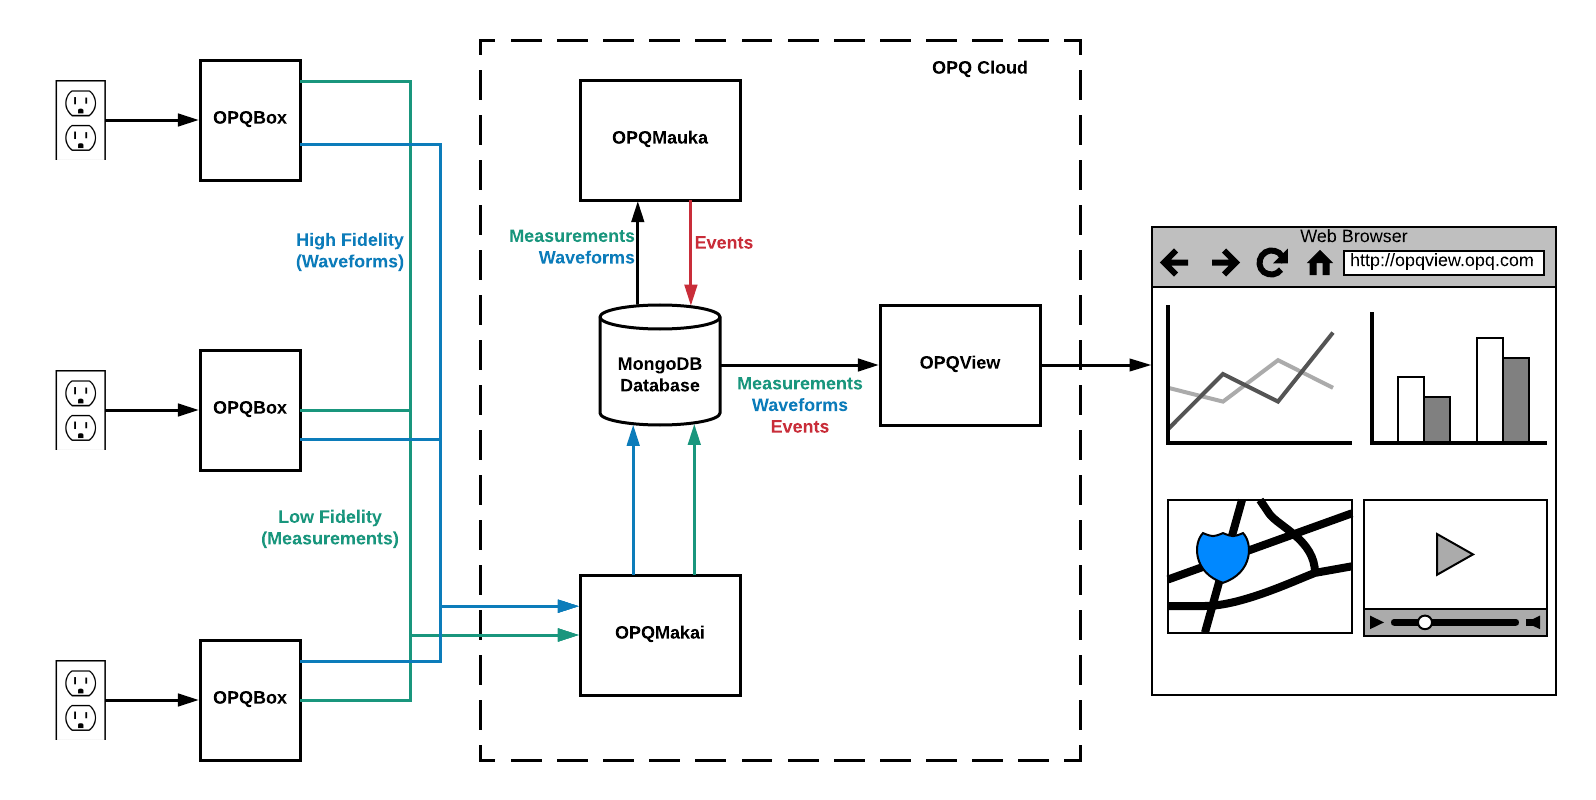
\includegraphics[width=5in]{images/architecture/system-diagram.png}
\caption{High level system architecture of an OPQ Sensor Network}
\label{fig:architecture}
\end{figure}


Figure \ref{fig:architecture} illustrates how these components work together to take information from wall outlets (on the left side) to the display of analyses in a browser (on the right hand side).  First, OPQ Boxes analyze power from wall outlets, and send low fidelity measurements to OPQ Makai. OPQ Makai analyzes low fidelity measurements, and requests high fidelity waveforms when desirable. Both measurements and waveforms are saved in a MongoDB database. OPQ Mauka analyzes low and high fidelity data, and creates "events" to represent anomalies. OPQ View notifies users of events and allows them to drill down into low and high fidelity data.

OPQ Makai, OPQ Mauka, and OPQ View are all cloud-based software services that collectively form a single "instance" with respect to data transmission, storage, analysis, and visualization. We refer to this collection of software-side components as OPQ Cloud. Every OPQ Box connects to a single instance of an OPQ Cloud. It is possible to have multiple OPQ Cloud instances. For example, a company might install an OPQ Cloud instance behind their firewall along with OPQ Boxes to provide a private mechanism for collecting and analyzing power quality data.

This architecture has a number of benefits. The combination of low and high fidelity data reduces both network overhead and storage requirements, which increases the scalability of the system in terms of the number of OPQ Boxes that can be tied to a single OPQ Cloud instance. OPQ Makai and OPQ Mauka have a plugin architecture, making it easier to extend their functionality to incorporate new triggers for high quality data (in the case of OPQ Makai) and new events and analyses (in the case of OPQ Mauka). Finally, the open source licensing of both hardware and software makes it possible to incorporate new ideas, bug fixes, and enhancements from technologists across the power quality community.

\section{Information Architecture}
\label{sec:information-architecture}

OPQ's "information architecture" is designed to facilitate the process of generating actionable, useful insights into the nature of the electrical grid starting with the data collected from a wall outlet. The information architecture must address several requirements. First, it must support analyses that require access to high fidelity data, which in the case of power quality is wave form data produced by sampling the wave form 256 times per cycle, which means there are approximately 1.3 billion data points generated per day per OPQ Box. Second, for typical grids that are generally stable, only an extremely small fraction of these data points are actually interesting. Third, as will be discussed in more detail later, what constitutes ``interesting'' data in one box might be dependent upon the state of data in other nearby boxes. Finally, network and storage limitations preclude a solution in which all data is sent from OPQ Boxes to the cloud, and so the information architecture must provide a ``smart'' mechanism for identifying data of interest on the boxes, as well as discarding data in the cloud if it is found to be not useful.

To address these requirements, the OPQ information architecture is organized as a five layer pyramid as summarized in Table \ref{fig:information-architecture}. This table illustrates an important conceptual feature of the OPQ information architecture called ``TTL'', or Time To Live. The OPQ information architecture implements an active, ``use it or lose it'' approach to information management, in which a data item must either be associated with a higher level of the system within its Time To Live, or else it will be automatically deleted. So, for example, the high fidelity waveform data on an OPQ Box have a TTL of one hour: if that data is not requested from a box by a higher layer in the information architecture within an hour of it being generated, it will be lost. Similarly, data points in the Measurement layer will be deleted after one day if they are not associated with an Event.

\begin{table}[H]
\caption{OPQ Information Architecture Levels}
\centering
%% \tablesize{} %% You can specify the fontsize here, e.g., \tablesize{\footnotesize}. If commented out \small will be used.
\begin{tabular}{llp{4in}}
\toprule
\textbf{Layer}	& \textbf{TTL}	& \textbf{Purpose}\\
\midrule
Box		& 1 hour			& Collects and holds a rolling one hour window of "high fidelity" wave form data for a single location.\\
Measurement		& 1 day			& Measurements provide "low fidelity" summary statistics regarding four power measurements (Frequency, Voltage, THD, Transients). \\
Event & 1 month & When OPQ Cloud's Makai service detects non-nominal values in the stream of Measurements, it can decide to request an ``event'': wave form data from one or more boxes for a specific time interval (typically just a second or so). \\
Incident & 6 months & An Incident is created when an Event satisfies a standard (such as IEEE 1159, ITIC, or SEMA) for a significant power quality problem.\\
Phenomena & 1 year & Phenomena classify Incidents when they are predictable and/or have a known causal explanation. \\
\bottomrule
\end{tabular}
\label{fig:information-architecture}
\end{table}

Let's now discuss how information moves through these levels.

The bottom layer of the information architecture is called Box, and represents all of the OPQ Box hardware devices in an OPQ sensor network. Each box maintains onboard storage of the latest hour of high quality waveform data in a circular buffer.

Approximately once a second, each Box sends a Measurement data object to the sensor network's cloud services, which we refer to in aggregate as OPQ Cloud. Measurements are the second layer of the information architecture, and provide "low fidelity" summary statistics regarding four power quality measurements (Frequency, Voltage, THD, and Transients). Measurements give OPQ Cloud basic situational awareness of the grid without the overhead of transmitting, storing, and analyzing high fidelity wave form data. Measurements exist for one day, though a daily roll-up of Measurement summary statistics called "Trends" persists longer.

When OPQ Cloud's Makai service detects non-nominal values in the stream of Measurements, it can decide to request wave form data from one or more boxes for a specific time interval (typically just a second or so). Note that Makai only has one hour to request high fidelity wave form data before it is lost.

Not every non-nominal power data value is significant, or in other words, meaningful for gaining insight into the grid. Over the years, the power community has developed a variety of standards (IEEE 1159, ITIC, SEMA, etc.) for characterizing significant power quality events. OPQ Cloud's Mauka service provides classification algorithms to analyze each Event to see if it satisfies any of the standards for significance. If so, an Incident is created, indicating that a significant PQ event has occurred at a specific time in a specific location. Each Incident can also be annotated with context, which is additional information about the environment or other physical factors present at the time and location of this incident. Context can be manually provided by users or automatically associated with Incidents through APIs to online services.

All of the prior levels represent behaviors of a individual Boxes in a single location at a given point in time. This final level of OPQ's information architecture is premised on the idea that insightful, actionable information results from the ability to either explain or else predict multiple Incidents. First, a Phenomena can be created in order to collect data from multiple Incidents with a common cause. An example of this form of phenomena is "the voltage drop experienced by all boxes in Kailua on 5/22/18 at 1:03pm was caused by a transformer trip at the Kailua substation." Second, a Phenomena can collect data from multiple Incidents in order to predict future Incidents. For example, "when winds exceed 40 knots in Kahuku, data from prior Incidents leads to the prediction that there will be a voltage surge of approximately 5V for approximately 3 seconds in all boxes located within 1 mile of Kahuku."





\section{Misc. Literature Quotes}

In February 2014 on the Big Island, the utility reports that 10\% of its circuits hit unstable levels \cite{trabish_solar_2014}.

Photovoltaics affect power quality by introducing harmonics \cite{anurangi_effects_2017}. The power feed-in of PV generation in rural low-voltage grids can influence power quality (PQ) as well as facility operation and reliability \cite{rita_pinto_impact_2016}.

Models, not actual installations \cite{anurangi_effects_2017,bayindir_effects_2016,farhoodnea_power_2012,shafiullah_experimental_2014}. Or data taken for only one week \cite{kucuk_assessment_2013}.

``across all business sectors, the U.S. economy is losing between \$104 billion and \$164 billion a year to outages and another \$15 billion to \$24 billion to PQ phenomena'' \cite{elphick_summary_2015} India lost more than \$9.6 billion in 2008 due to power quality, and Europe lost \$150 billion per year \cite{laskar_power_2012}.

A study of the island of Porto Santo in Portugal found that intermittent nature of installed photovoltaic and wind energy could result in a potential drop in frequency of 12 Hz, lasting as long as 7 seconds \cite{delgado_solutions_2011}.

Reduced input voltage can cause excessive power supply heat dissipation, resulting in reduced mean time between failures (MTBF). In addition, rectifiers and DC-to-DC converter switching transistors draw high-peak currents, which raise their junction temperatures. These temperature excursions take a toll on semiconductor longevity. High input voltage can also puncture a power supply's rectifier and switching transistor junctions, causing MTBF reduction and eventual breakdown. High-voltage transients lasting microseconds can permanently wreck the power supply and its electronic equipment load. \cite{dedad_when_2008}.

Solar panels connected to low voltage networks will result in over-voltages, the switching frequency of the converters in wind turbines causes high-frequency signals flowing into the grid, and harmonics are generated by EV chargers. \cite{zavoda_power_2018}

OPQ Boxes do not collect PQ measures such as phase angle or reactive power.

The main challenge is to go beyond manual methods based on the intuition and heuristics of human experts...it is crucial to develop the machine intelligence needed to automate and scale up the analytics on billions of PMU measurements and terabytes of data on a daily basis and in real time. \cite{mohsenian-rad_distribution_2018}



% Bibliography
\reftitle{References}
\bibliographystyle{mdpi}
\bibliography{opq}

\end{document}

